% *********************************************************************
% © 2010–2023 Jeremy Sylvestre
%
% Permission is granted to copy, distribute and/or modify this document
% under the terms of the GNU Free Documentation License, Version 1.3 or
% any later version published by the Free Software Foundation; with no
% Invariant Sections, no Front-Cover Texts, and no Back-Cover Texts. A
% copy of the license is included in the appendix entitled “GNU Free
% Documentation License” that appears in the output document of this
% PreTeXt source code. All trademarks™ are the registered® marks of
% their respective owners.
%
% *********************************************************************

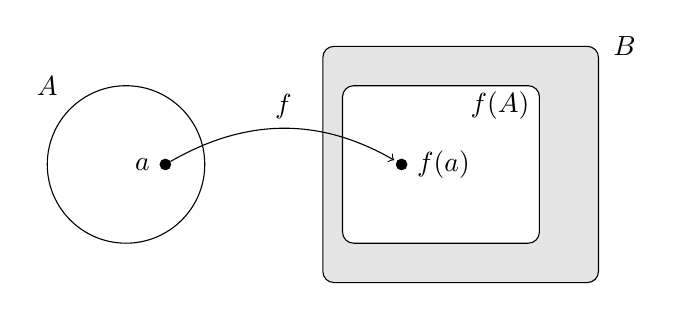
\begin{tikzpicture}[
	vertex/.style={ circle, draw, very thin, fill, inner sep=0pt, minimum size=4pt },
	vertexg/.style={ black!40!white, circle, draw, very thin, fill, inner sep=0pt, minimum size=4pt },
	vertexo/.style={ circle, draw, very thin, inner sep=0pt, minimum size=4pt }
]

\draw[rounded corners,fill=black!10!white]
  (0.5,-1.5) rectangle (4,1.5);
\draw[rounded corners,fill=white] (0.75,-1) rectangle (3.25,1);
\draw (-2,0) circle (1cm);
\node at (2.75,0.75) {$f(A)$};
\node at (-3,1) {$A$};
\node at (-1.5,0) (a) [vertex,label=left:$a$] {};
\node at (1.5,0) (b) [vertex,label=right:$f(a)$] {};
\draw[->,shorten >=1pt] (a) to [out=30,in=150] node[above] {$f$} (b);
\node at (4.33,1.5) {$B$};

\end{tikzpicture}
